
%%% Local Variables: 
%%% mode: latex
%%% TeX-master: "russian"
%%% End: 

\section{游戏的结构}


程序用Gtk的面向对象的方式设计,有三个类实现,Diamone是单方块类,实现了单方块的显
示、移动,Mass是形状类,实现了7种俄罗斯方块形状的显示、移动、转换,DataBase是数据
库类,实现所有数据存取、处理,主程序调用Mass类、DataBase类。


\begin{shell}
\begin{verbatim}                         
        +--------------+ 4               1+-------------+           
        |   Diamond    +o-----------------+     mass    +           
        +--------------+            +----o+-------------+           
       russian_diamond_leftmove     |  2  russian_mass_leftmove     
       russian_diamond_rightmove    |     russian_mass_rightmove    
       russian_diamond_downmove     |     russian_mass_downmove     
                                    |     russian_mass_translate    
                                    |                               
                        1           |                               
        Russian主函数---------------+                               
                                    |                               
                                    |       russian_db_init         
                                    |       russian_db_repair_matrix
                                    |   1   +-----------+
                                    +------o+ DataBase  +
                                            +-----------+
\end{verbatim}
\end{shell}


\subsection{主程序}


主程序中绘制程序界面,实现事件回调函数;在expose-event事件中调
用gdk\_draw\_drawable,把内存图形显示到绘图区域;在key-press-event事件中调
用Mass类的russian\_mass\_leftMove、russian\_mass\_rightMove等方法响应上下左右按键操
作;在定时事件中调用DataBase类和Mass类的方法,实现俄罗斯方块的定时下落。

主程序中界面由运行区、后备区、开始按键、暂停按键组成,方块毎隔500mS下落一行;程序
中用table布局,界面为左右结构左边是运行区,右边是后备区、开始按键、暂停按键,参
见\pageref{fig:russian}页图\ref{fig:russian};运行区显示的是当前的形状,后备
区中显示将要在运行的形状,如当前形状下落到底,后备形状就成为当前形状,后备区随机
生成一个后备形状;程序中后备区和开始按键放入GtkVBox控件中,用vbox和alignment实
现,右边控件紧缩在一起的效果,下面的一段程序:

\begin{figure}[htbp]
  \centering
  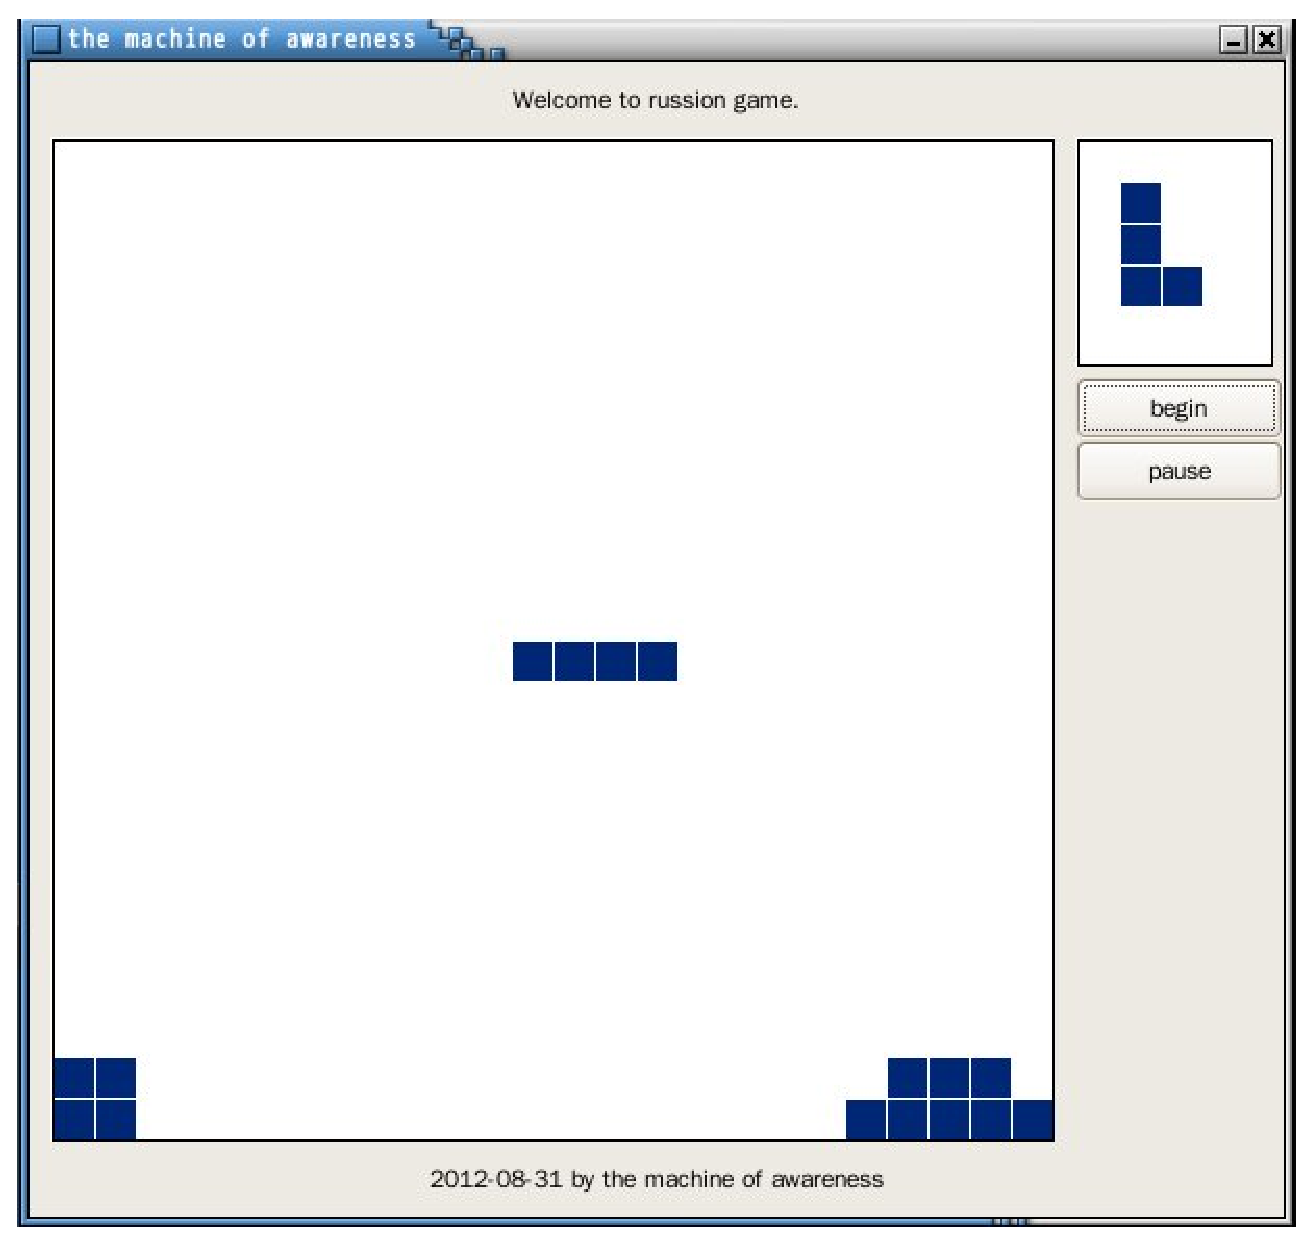
\includegraphics[width=3.5in]{images/russian}
  \caption{游戏界面}
  \label{fig:russian}
\end{figure}

\begin{shell}
\begin{verbatim}
  // 这里,用vbox和alignment实现,右边控件紧缩在一起的效果
  // vbox中包含的widget
  vbox = gtk_vbox_new(FALSE, 5);
  // s_drawArea
  // 设置s_drawArea的expose事件,在事件中显示图形
  g_signal_connect(s_drawArea, "expose-event", G_CALLBACK(on_s_expose), draw_info);
  // 实现右边控件紧缩在一起的效果,vbox的yoptions一定为要GTK_FILL
  gtk_table_attach(GTK_TABLE(table), vbox, 1, 2, 1, 2, 0, GTK_FILL, 0, 0);    
  gtk_widget_set_size_request(s_drawArea, 95, 110);
  gtk_box_pack_start(GTK_BOX(vbox), s_drawArea, FALSE, FALSE, 0);
  // button
  button = gtk_button_new_with_label("begin");
  g_signal_connect(button, "clicked", G_CALLBACK(on_begin), pause_button);
  gtk_widget_set_size_request(button, 100, 30);
  gtk_box_pack_start(GTK_BOX(vbox), button, FALSE, FALSE, 0);
  // alignment
  alignment = gtk_alignment_new(0, 0, 0, 0);
  gtk_widget_set_size_request(pause_button, 100, 30);
  gtk_container_add(GTK_CONTAINER(alignment), pause_button);
  // 实现右边控件紧缩在一起的效果,alignment的yoptions一定为要GTK_FILL|GTK_EXPAND
  gtk_table_attach(GTK_TABLE(table), alignment, 1, 2, 2, 3, 0, GTK_FILL|GTK_EXPAND, 0, 0);
\end{verbatim}
\end{shell}

软件用键盘控制运行区的形状,形状可以左移、右移、下移、变形,分别用键盘的左、右、
下、上控制,软件还支持emacs操作方式,左移(C-b),右移(C-f),下移(C-n),变形
(C-p),直接移到最左边(C-a),直接移到最右边(C-e)。

\subsection{Diamond类}

Diamond类实现俄罗斯方块最基本的组成单元,单个方块的显示、清除、向左右下移动;方块
宽度为20pt的正方形,中间19pt的实心正方形,周围留有1pt,这样显示多个方块时,之间就
有1pt的间距;程序的方块有两种,一种是在容器中显示,称为主用方块,一种在备用区显
示,称为备用方块;主用方块的位置信息是虚拟的,横坐标范围是-12$\sim$11,纵坐标范围
是0$\sim$23,对应实际横坐标范围0$\sim$460,纵坐标范围0$\sim$460,显示方块时要进行
位置信息和坐标之间进行转换。

Diamond类中display方法显示方块时,绘图参数GdkGc是GtkWidget下的GtkStyle类中定义
的fg\_gc[GTK\_STATE\_INSENSITIVE],并定义为深蓝色;Diamond类中display方法清除方块
时,绘图参数GdkGC是GtkWidget下的GtkStyle类中定义的white\_gc;方块显示成深蓝色,清
除后为白色。

\subsection{Mass类}

形状类(Mass)包含4个方块类,毎个方块都有自己的位置;4个方块根据相对位置组成7种不同
的形状,形状类型由type表示,形状还可以变形,当前变形的编号由tran\_type。

形状可以左
移(russian\_mass\_leftMove),右移(russian\_mass\_rightMove),下移
(russian\_mass\_downMove),变形(russian\_mass\_translate),形状中的方块位置发生
相应的变化;毎次操作前都要判断执行完操作后,方块的位置是否合法,如不合法,不能执
行这个操作,比如形状移动到容器最左边,再执行左移是无效的。

\subsection{DataBase类}

DataBase类包含数据,是一个单例类,包含绘图信息(data\_base.h),游戏运行信息;绘图信息是绘图时
所用到的所有数据,包含绘图相关的绘图区对象(area),内存绘图区对象(pixmap),运行中
的形状(mass);游戏运行信息是游戏运行用到的数据,包含容器数组,游戏状态(暂停/结束)。

DataBase类定义了7种形状位置信息(\_initdat),变形信息(\_muldat),毎个形状初始化时都要调
用russian\_db\_init\_mass,根据形状的类型将位置信息数据辅给形状中的方块,毎个形状变形时要调
用russian\_db\_do\_tranlate,根据变形信息变换形状中的方块位置。

DataBase类是所有数据操作的中心,当形状显示时,需设置容器标
记(russian\_db\_set\_mark);当形状下落到容器底部时,需分析容器,清除已满的
行(russian\_db\_repair\_maxtrix);运行形状是否可以移动由容器边界和标记决
定,都在DataBase类中判
断。(russian\_db\_is\_leftmove、russian\_db\_is\_rightmove、russian\_db\_is\_downmove、
russian\_db\_is\_translate)


形状位置信息(\_initdat),是7种形状初始位置信息,如\_initdat[1],数
据:0,0,0,1,0,2,0,3,说明这个形状的4个方块位置
是(0,0),(0,1),(0,2),(0,3);用Diamond类的display方法显示出来,是长条形状。


